\documentclass[_main.tex]{subfiles}
 
\begin{document}

\section*{Genetic variation at a point locus} 
\label{main_point_locus}

Now that we have a way to estimate time to coalescence, we can use this to estimate levels of genetic variation in the parasite population.  We start by focusing on an imaginary locus in the parasite genome.  We refer to a single nucleotide position as a \textit{point locus} and we define a \textit{haplotype locus} as a sequence that extends over multiple nucleotide positions (see glossary figure \ref{fig:supp_graph_17}).  A haplotype locus can undergo recombination whereas a point locus cannot.  We shall discuss haplotype loci in the next section but here we focus on point loci, so we can ignore recombination for the present.

\begin{figure}[h!]
\centering
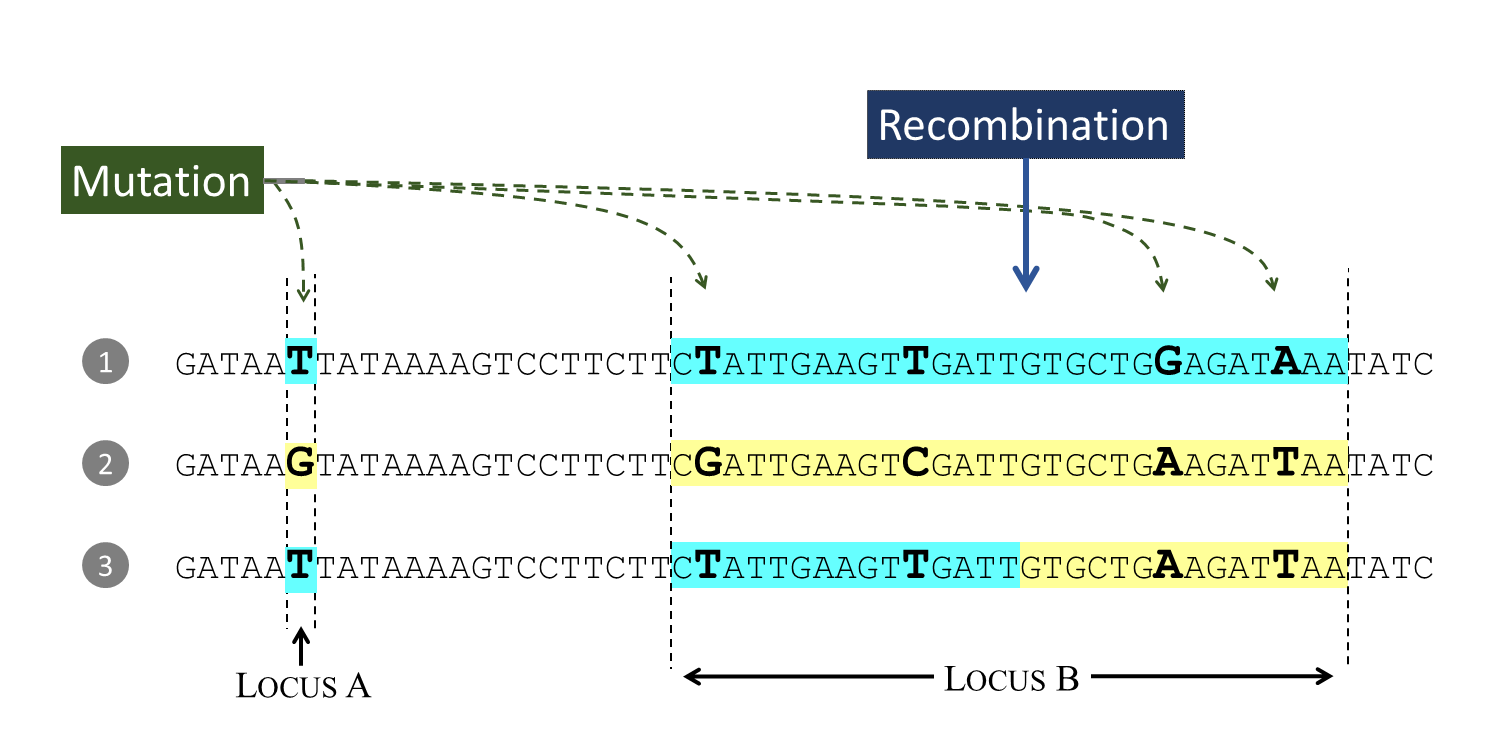
\includegraphics[width=12cm]{181001a_alleles.png}
\caption{\textbf{We measure heterozygosity by comparing the genome sequence of two alleles at a locus}. An allele is an instance of the parasite genome and a locus is a specific location in the genome.  Here we see three alleles at two loci: locus A is a single nucleotide position (we call this a point locus) and locus B extends over multiple nucleotide positions (we call this a haplotype locus).  Both loci have been affected by mutation, and locus B has also been affected by recombination.}
\label{fig:supp_graph_17}
\end{figure}

We say that alleles are \textit{homozygous} if they have the same DNA sequence, and that they are \textit{heterozygous} if they have different DNA sequences.  We define \textit{homozygosity} as the probability that two randomly sampled alleles at a particular locus are homozygous, and \textit{heterozygosity} as the probability that they are heterozygous.  Following convention we denote homozygosity by $G$ and heterozygosity by $H$, where $H = 1 - G$.

Imagine that we sample two alleles at a point locus and trace their lineages back in time until they coalesce.  Let $u$ be the mutation rate per generation at this locus and let \textbf{T} be a random variable representing time to coalescence of the two lineages.  The two alleles must have the same DNA sequence if neither lineage is affected by mutation from the time of sampling to the time of coalescence, so as described in Methods section \ref{supp_point_locus} we can obtain the expectation of heterozygosity

\begin{equation*}
E\{ H \} = 1 - \sum_{i=1}^\infty \Pr \{ \textbf{T} = i \} \times (1-u)^{2i}
\label{eq:main_het_pdf}
\end{equation*}

Let $T_C$ be the mean time to coalescence measured in generations.  If $u$ is sufficiently small (say $<10^{-5}$) we can safely ignore factors of $u^2$ and above to make the approximation

\begin{equation}
H \approx 2 u T_C
\label{eq:main_het_approx}
\end{equation}

\paragraph{Mechanisms of mutation at a point locus.} There are various mechanisms of mutation, each causing a characteristic type of genetic varation.  They include substitutions, insertions, deletions and structural rearrangements.  Here we focus on single nucleotide substitution, the mutational process that causes a very common type of genetic variation known as a single nucleotide polymorphism (SNP).  SNPs naturally correspond to point loci and are convenient for analysis because they are relatively easy to ascertain using current genome sequencing technologies.  We can therefore use the rate of single nucleotide substitution as a form of molecular clock as we track lineages back in time.

\paragraph{Single nucleotide substitution rate $\mu$.}  Let $\mu$ be the probability of single nucleotide substitution occuring at a point locus during one generation of the transmission graph.  \textit{In vitro} studies of \textit{P. falciparum} clone trees have estimated the probability of a single nucleotide substitution to be in the region of $10^{-9}$ to $10^{-10}$ per nucleotide during each 48-hour cycle of replication within erythrocytes \cite{Bopp2013,Claessens2014,Hamilton2016}.  Here we shall use the rather conservative estimate of $1.2 \times 10^{-10}$ per nucleotide per day based on the largest of these studies \cite{Hamilton2016}.  We do not know the rate of mutation at other stages of the life cycle, e.g. when parasites replicate within the mosquito or in the human liver, but let us assume that $1.2 \times 10^{-10}$ per nucleotide per day is representative of the entire life cycle.  If we also assume that the serial interval of transmission $\tau$ is 3 months, we obtain an estimate of $\mu \approx 1.1 \times 10^{-8}$ per generation.  

\paragraph{Nucleotide diversity $\pi$.}  We define nucleotide diversity as the probability that two alleles are heterozygous at a random nucleotide position in the genome, and we denote this by $\pi$.  The value of $\pi$ will vary from population to population but we can measure it using genome sequence data, and it provides a direct estimate of the genome-wide average of heterozygosity for all point loci.  This provides a starting point for analysis of parasite population history as it allows us to estimate the mean time to coalescence.  If we take equation \ref{eq:main_het_approx} and substitute $\pi$ and $\mu$ respectively for $H$ and $u$, we obtain

\begin{equation}
T_C \approx \frac{\pi}{2 \mu}
\label{eq:main_Tc_pi}
\end{equation}

Measuring $\pi$ in a parasite population is straightforward in principle: we randomly sample parasites from the population, obtain their genome sequences, and analyse the number of pairwise differences between individual genome sequences. In practice, the definition of $\pi$ needs to be modified slightly to make these empirical measurements consistent with our definition of $\mu$, and to exclude potential sources of error and bias.

%%%%%%%%%%%%%%%%%%%%%

\paragraph{Nucleotide diversity of the global parasite population.} 
\label{main_global_diversity_1}

From large genome sequencing studies of thousands of \textit{P. falciparum} samples from around the world, we can get an estimate of global, regional and local levels of nucleotide diversity  \cite{MalariaGEN2021,MalariaGEN2023}.  There are some technical caveats about the precision of these estimates, as discussed in Methods section \ref{supp_global_pi}, but for present purposes we can use $\pi \approx 4 \times 10^{-4}$ as a first approximation for the global parasite population.  This estimate is obtained by analysis of coding SNPs as opposed to other types of genetic variation.  It is restricted to SNPs because our estimate of $\mu$ is based on the rate of single nucleotide substitution.  It excludes SNPs in non-coding regions because, in the case of \textit{P. falciparum}, these are error-prone due to many tandem repeat sequences.  

%When we measure genetic diversity, we need to specify the population that we are sampling from. Following convention we attach subscripts to $H$ and $\pi$ to indicate where the sample resides within a hierarchical population structure:

%\begin{itemize} [noitemsep]

%\item[-] $H_T$ and $\pi_T$ refer to the global population (\textsc{t} stands for total)

%\item[-] $H_R$ and $\pi_R$ refer to a regional population, e.g. West Africa

%\item[-] $H_S$ and $\pi_S$ refer to a local population (\textsc{s} stands for sub-population)

%\item[-] $H_W$ and $\pi_W$ refer to the parasite population within an individual host

%\end{itemize}

If $\pi \approx 4 \times 10^{-4}$ and $\mu = 1.1 \times 10^{-8}$, then equation \ref{eq:main_Tc_pi} tells us the mean time to coalescence for two alleles sampled at random from the global parasite population is approximately 18,000 generations.  This is equivalent to 4,500 years since we are assuming that each generation has a duration $\tau$ of 3 months.  If we specified a different value for $\tau$ this would change our estimates of $\mu$ and of $T_C$ measured in generations, but it would still give us a mean coalescence time of approximately 4,500 years.

\paragraph{Transmission parameters compatible with global levels of nucleotide diversity.}  Knowing the single nucleotide substitution rate $\mu$, we can use Markov chain simulation of coalescence times to explore what combinations of transmission parameters would be compatible with the observed levels of nucleotide diversity in the global parasite population.  Undoubtedly the transmission parameters have varied considerably over the past few thousand years, but for the purpose of illustration we shall assume here that they are constant over time.   

As an example, the combination of $N_h = 18764$, $Q = 1$, $\chi = 0$ would give $\pi = 4 \times 10^{-4}$.  As we noted in the previous section, a transmission graph with $Q = 1$, $\chi = 0$ is equivalent to a Wright-Fisher population of $N_h$ haploid individuals.  In other words, if we applied the Wright-Fisher model to these data, we would obtain an effective population size of 18,764 haploid individuals.

Another possible combination is $N_h = 3269$, $Q = 10$, $\chi = 1$.  This gives the same value of nucleotide diversity in the general parasite population but a much higher level of within-host diversity, both because transmission chains cross more frequently, and also because the transmission bottleneck is not so tight.  Other examples that lie in between these two extremes are shown in table \ref{table:comb_of_trans_var}.

 \begin{table}[h!] 
\centering
\small{
\begin{tabular}{c c c c c c c c} 
\hline \\
$\chi$ & $Q$ & $N_h$ & $\pi_T$ & $\widehat{\pi}_W$ \\ [0.5ex] 
\hline \\
0 & 1 & 18,764 & $4.0 \times 10^{-4}$ & $2.2 \times 10^{-8}$ \\ [2ex]
0 & 10 & 18,754 & $4.0 \times 10^{-4}$ & $2.2 \times 10^{-7}$ \\ [2ex]
0.5 & 1 & 18,764 & $4.0 \times 10^{-4}$ & $2.0 \times 10^{-4}$ \\ [2ex]
0.5 & 10 & 5,568 & $4.0 \times 10^{-4}$ & $3.1 \times 10^{-4}$ \\ [2ex]
1 & 1 & 18,764 & $4.0 \times 10^{-4}$ & $4.0 \times 10^{-4}$ \\ [2ex]
1 & 10 & 3,269 & $4.0 \times 10^{-4}$ & $3.7 \times 10^{-4}$ \\ [2ex]
\hline
\end{tabular}
}
\caption{\small{\textbf{Examples of transmission parameters giving $\pi = 4 \times 10^{-4}$.}  Here we use a simplistic model with constant population size to simulate the heterozygosity of a point locus.  The input parameters are $N_h$, $Q$ and $\chi$.  The results are $\pi_T$, the nucleotide diversity of the total parasite population, and $\widehat{\pi}_W$, the mean level of within-host nucleotide diversity.  \href{https://d-kwiat.github.io/gtg/nucleotide-diversity.html}{See worked example.}}}
\label{table:comb_of_trans_var}
\end{table}

It is evident from these observations that current levels of nucleotide diversity in the global parasite population have built up over thousands of years.  To put this in context, various lines of evidence indicate that \textit{P. falciparum} originated in Africa and underwent a major population expansion somewhere in the region of 10 to 50 thousand years ago \cite{Joy2003,Tanabe2010}.  Figure  \ref{fig:main_global_pi_1} illustrates this with a toy model in which nucleotide diversity gradually accumulates over time to reach a level of $\pi_T \approx 4 \times 10^{-4}$ in the total parasite population and of $\pi_W \approx 1 \times 10^{-4}$ in the within-host population. 

\begin{figure}[h!]
\centering
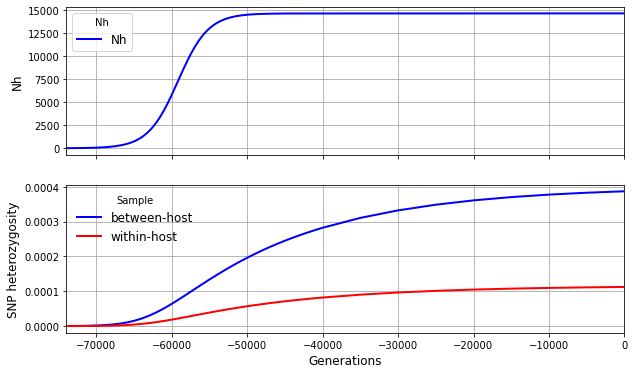
\includegraphics[width=12cm]{221123_global_SNP_het_2.png}
\caption{\textbf{A toy model of the global parasite population}.  In this very simplistic scenario, there is a major population expansion approximately 15 thousand years before the present, eventually reaching a plateau with $N_h = 14,660$, $Q = 3$ and $\chi = 0.2$ which is maintained over the past few thousand years.  Nucleotide diversity gradually increases to $\pi_T \approx 4 \times 10^{-4}$ in the total parasite population and $\pi_W \approx 10^{-4}$ in the within-host population.  To explore other simple scenarios see \href{https://github.com/d-kwiat/gtg/blob/main/species_history.ipynb}{this Jupyter notebook}.}
\label{fig:main_global_pi_1}
\end{figure}

\paragraph{Local levels of nucleotide diversity.} We might intuitively expect the nucleotide diversity of local parasite populations to be much lower than that of the global parasite population, but empirical measurements show that this is generally not the case.  Throughout much of Africa, the nucleotide diversity of the parasite population in a large village can be almost as high as that in the global population.  A modest reduction in nucleotide diversity is observed in parts of Southeast Asia where transmission intensity is much lower than Africa \cite{MalariaGEN2021,MalariaGEN2023}.  

As we shall discuss later, relatively low levels of ongoing migration across the global metapopulation can maintain high levels of nucleotide diversity in a local subpoulation.  It is quite possible that human migration out of Africa was a major factor in dispersing \textit{P. falciparum} around the world, but it is equally possible that the nucleotide diversity of local parasite populations has been maintained by human migration in the modern era, and these two possibilities are not mutually exclusive.  

Therefore we might not be able to learn much about local patterns of malaria transmission from levels of nucleotide diversity in the local parasite population, because these are greatly influenced by historical patterns of global population expansion and long-range dispersal.  However this background genetic diversity is extremely useful for other metrics that are more informative about recent local transmission, such as within-host heterozygosity, haplotype homozygosity and local population structure, as we shall discuss in the following sections.

\end{document}